
\section{Sistema Visual}

Descreva como funciona a fase de treino ou o tutorial do jogo que aparece na tela.


\section{Sistema de Controle}

O jogador deverá utilizar o teclado para controlar os personagens no jogo, por ser o método padrão de entrada em jogos para computadores. 

Para melhor entendimento, dividimos em três tipos de controle.

\subsection{Movimentação}

O jogador movimentará os personagens pelas teclas W, A, S, e D, sendo as ações respectivas, andar para frente, andar para a direita, andar para trás e andar para a esquerda por fim a tecla de espaço será utilizada para pulos. Optamos por esse mapeamento por ser um dos mais comuns entre os jogos para computadores, e dessa forma não confundir jogadores experientes.

\begin{figure}[!htb] \caption{\label{fig_tacladoMov}Teclas de Movimentação} \begin{center}
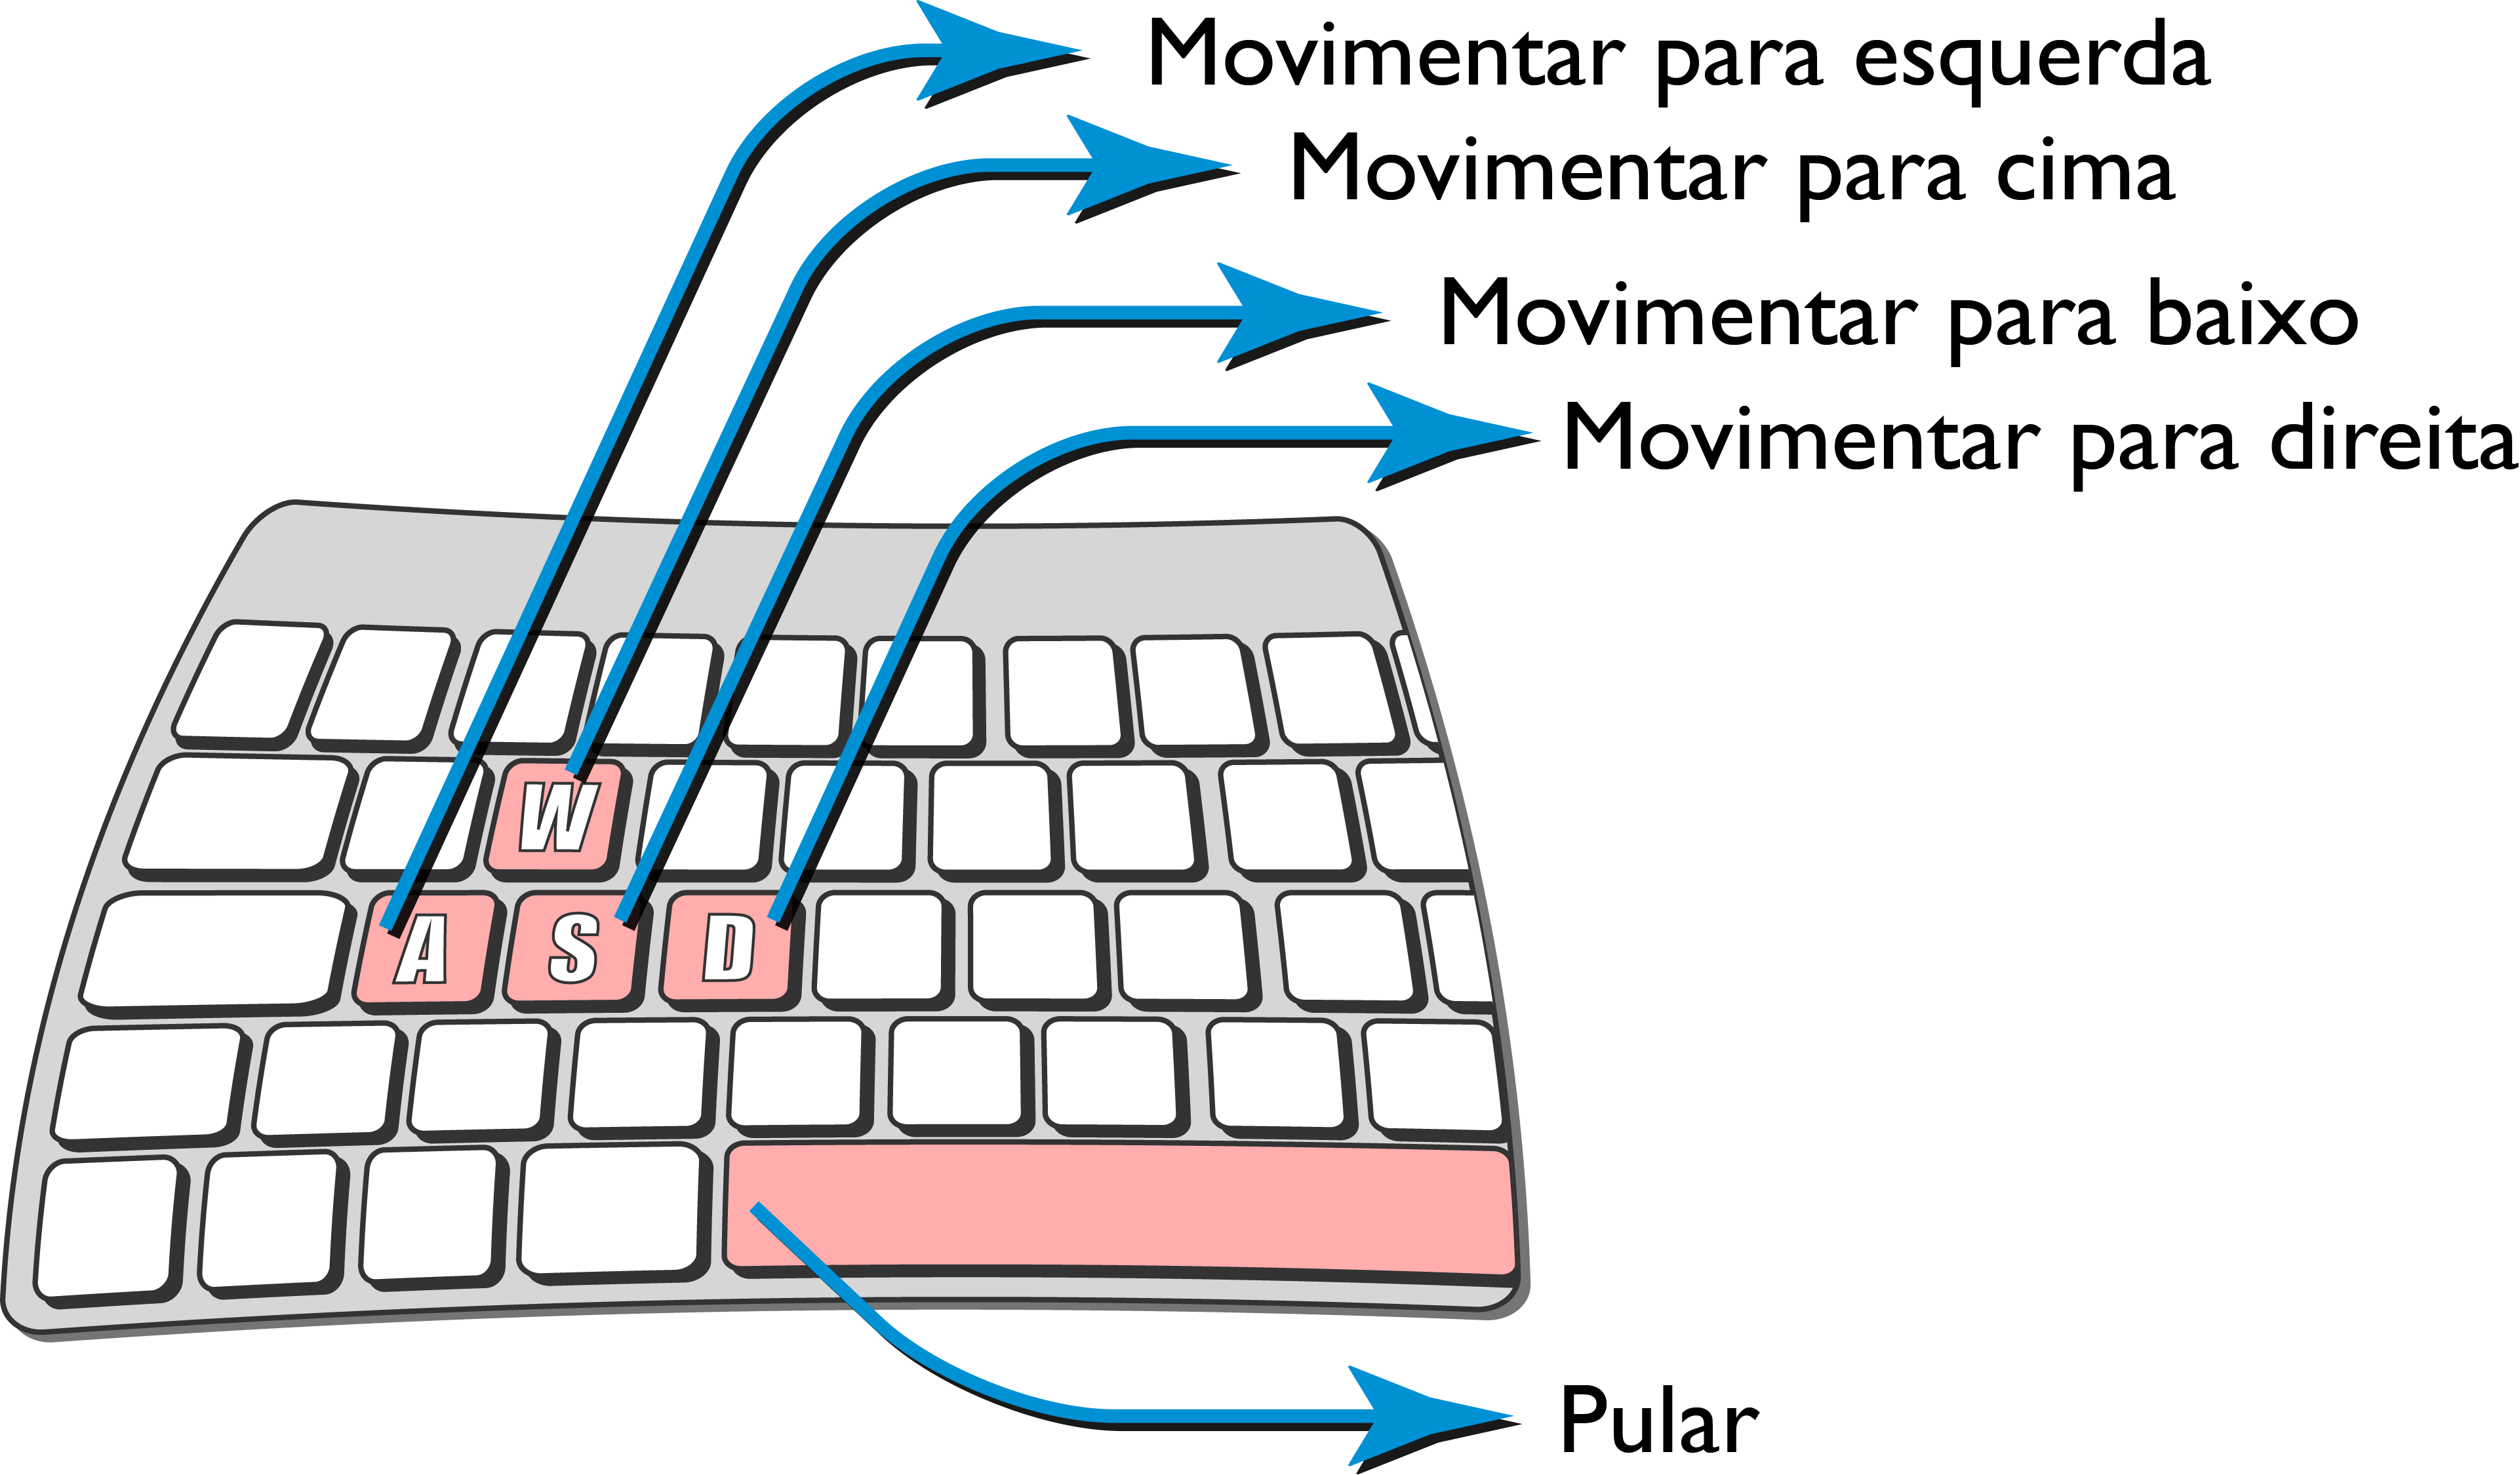
\includegraphics[width=0.5\textwidth]{imagens/tecladoMov.png} \end{center}
\legend{Fonte: Autoria Nossa} \end{figure}


\subsection{Troca de personagens}

A partir da quarta fase, o jogador poderá alternar entre os personagens que está controlando, para poder utilizar suas habilidades únicas, exitem duas formas de alternar entre personagens, utilizando a tecla Q que ira rotacionar entre os mesmos sempre na mesma ordem, temos a opção também de trocar diretamente para um dos personagens com as teclas Z, X, e C respectivamente.


\begin{figure}[!htb] \caption{\label{fig_tecladoTroca}Teclas de Troca de Personagem} \begin{center}
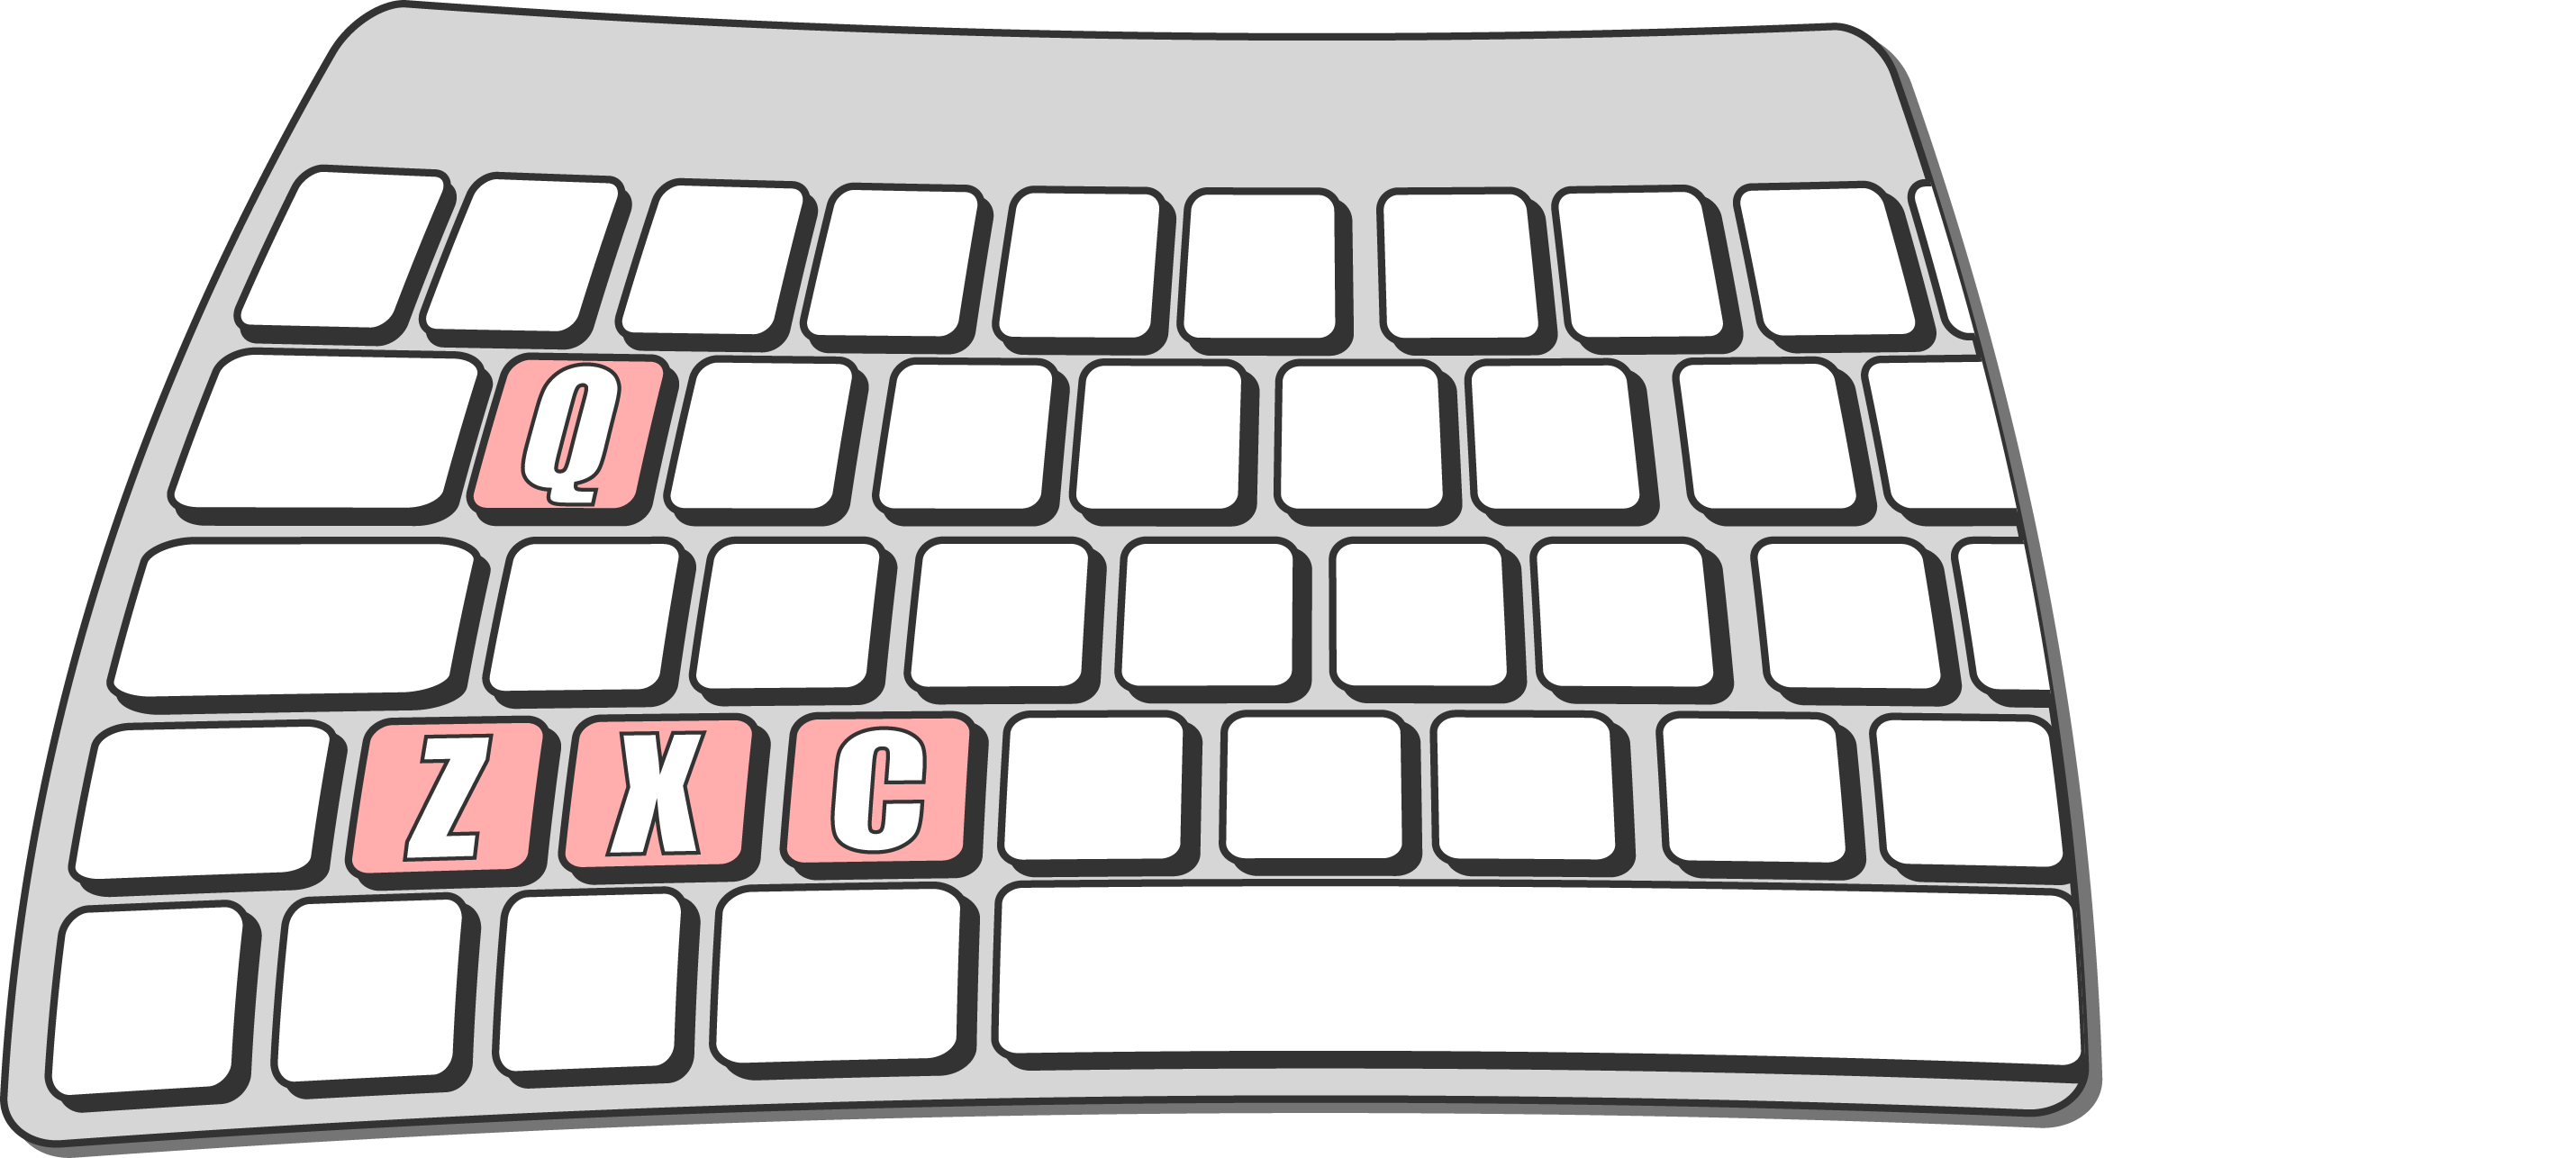
\includegraphics[width=0.5\textwidth]{imagens/tecladoTroca.png} \end{center}
\legend{Fonte: Autoria Nossa} \end{figure}

\subsection{Outras Interações}

Por fim, temos o sistema de uso de habilidades dos personagens que será feito pelas teclas 1, 2 e 3 na parte superior do teclado ficando responsáveis pela primeira segunda e terceira habilidades dos personagens respectivamente. 

Lembrando que cada personagem tem habilidades exclusivas, para maiores informações das habilidades específicas consulte a sessão 2.5 - Mecânicas

A tecla E, será utilizada para quaisquer outras ações não específicas dentro do jogo, como abrir porta, coletar itens, ativar mecanismos entre outros.

\begin{figure}[!htb] \caption{\label{fig_tecladoOutras}Teclas de Outras Interações} \begin{center}
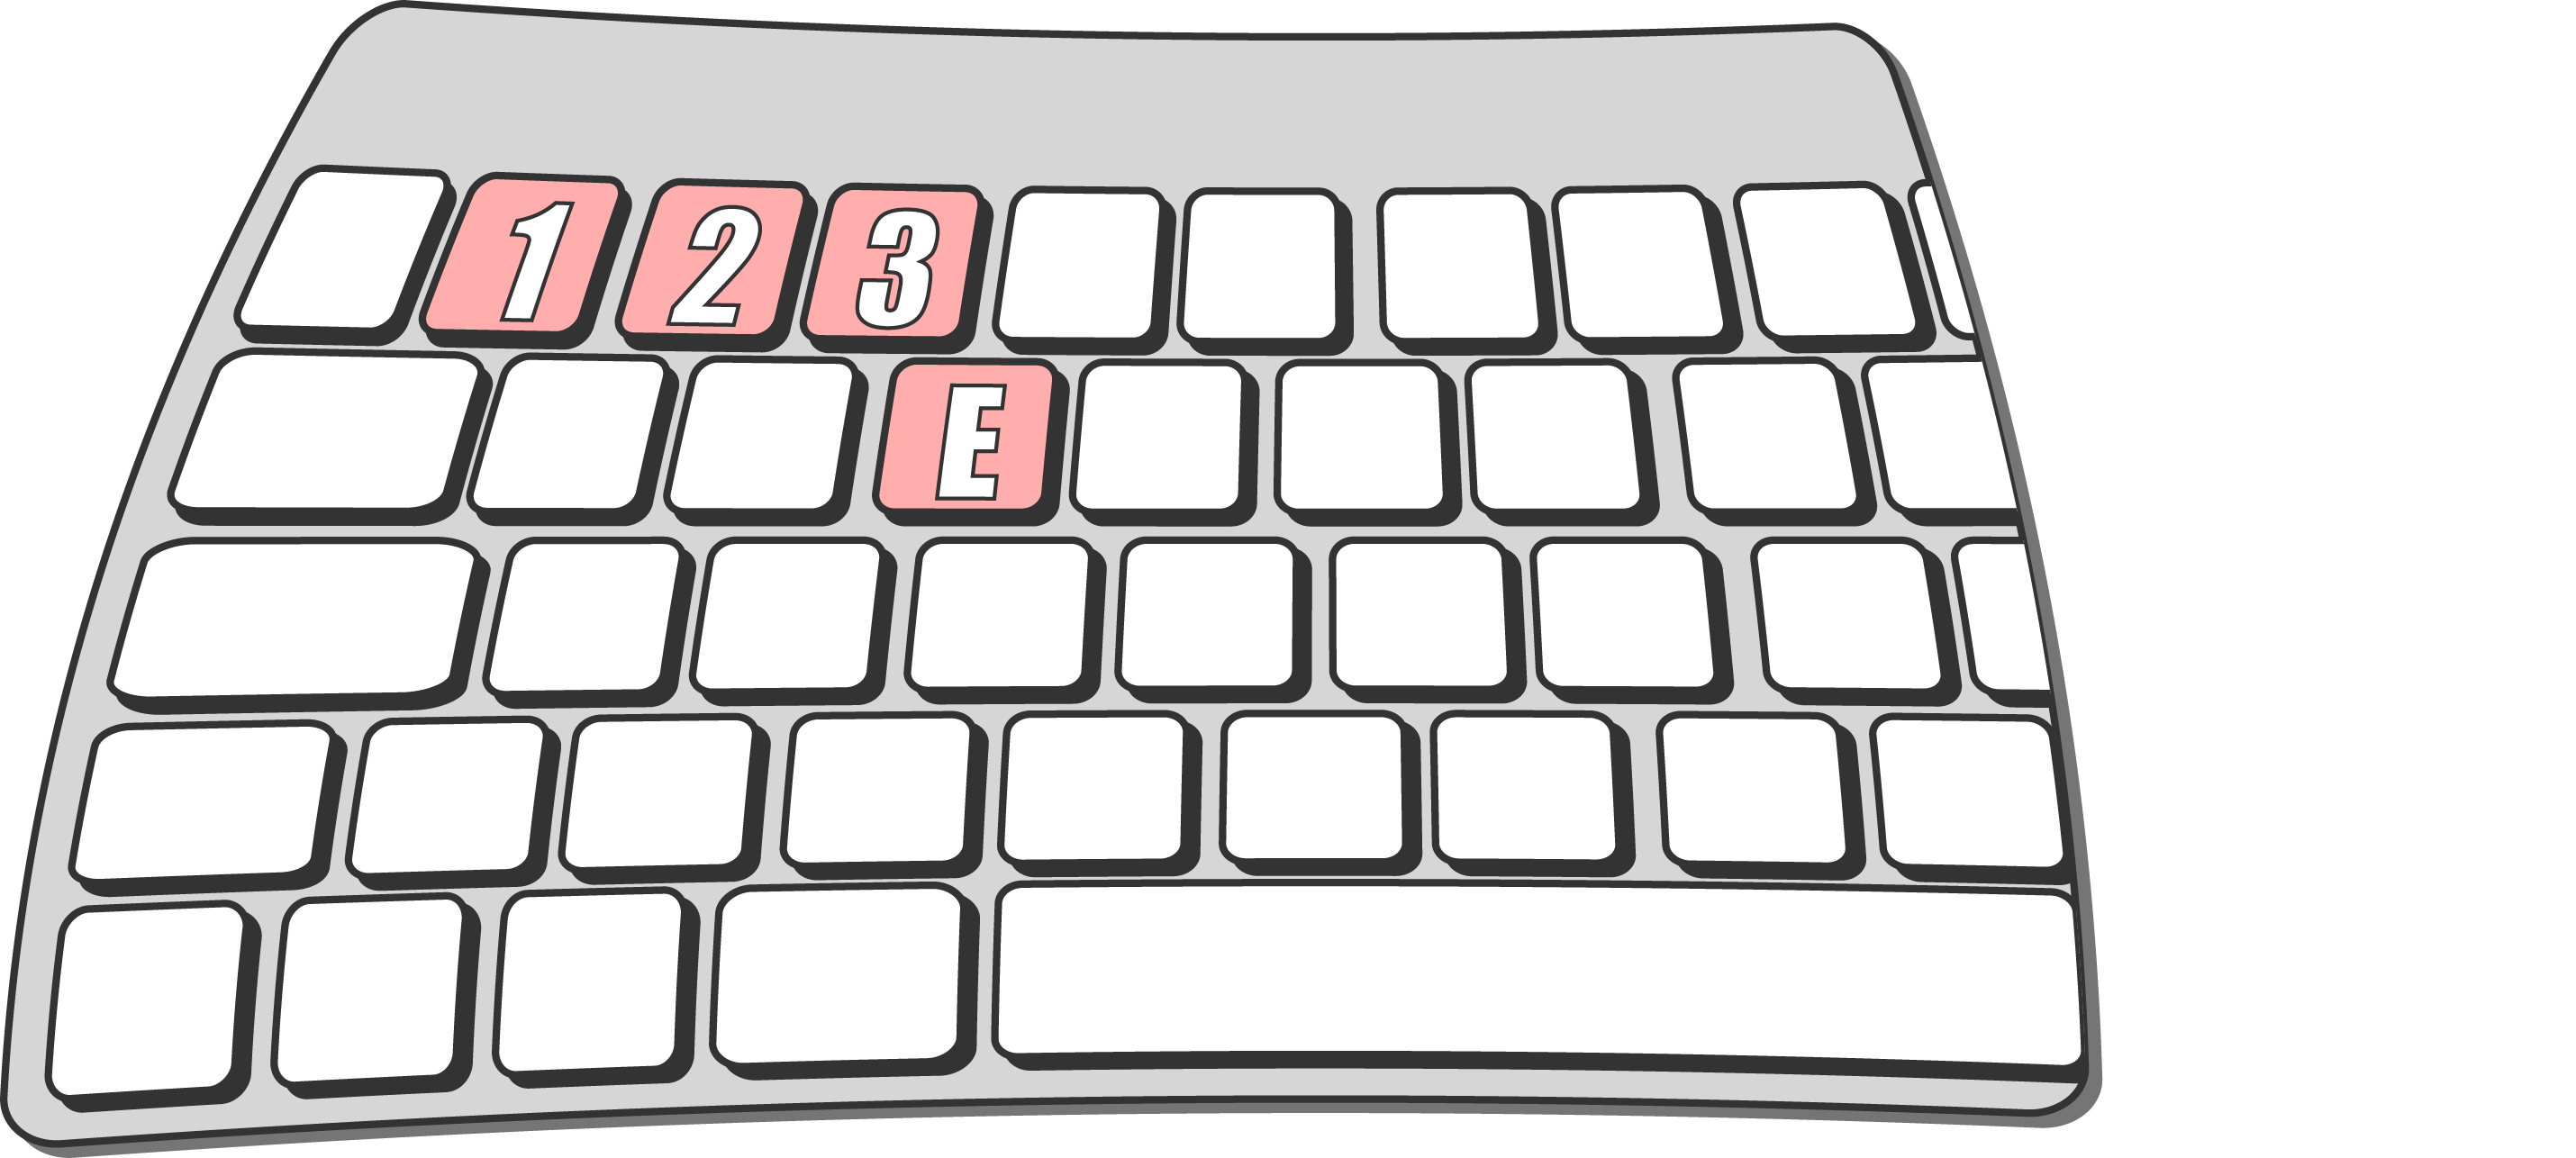
\includegraphics[width=0.5\textwidth]{imagens/tecladoOutros.png} \end{center}
\legend{Fonte: Autoria Nossa} \end{figure}



\section{Sistema de Ajuda}

Descreva (se houver) o sistema de dicas para o jogador caso ele não consiga continuar o jogo.